\chapter{Methods Review}
The purpose of the chapter is to provide a review of the main statistical methods used in this project.  See the cited references for a more thorough discussion on each topic.

\section{Poisson Regression}

Poisson regression is used to model count data and/or contigency tables. For example, Poisson regression can be used to model the number of incoming calls in a call center for different time segments throughout the day or, as in the case in this project, the number of car crashes on a segment of road.  Let $Y_i$ for $i=1,\dots,n$ denote a count response variable for the $i^{th}$ individual (e.g. road segment) and $n$ is the total number of individuals in the dataset (the sample size).  Furthermore, define $\vec{x}_i = (1,x_{i1},\dots,x_{iP})'$ to be a vector of $P$ covariates (and an intercept term) associated with $Y_i$. Poisson regression is a tool to estimate the relationship between $Y_i$ and $\vec{x}_i$.

As described in \citet{weisberg05}, the three main components of Poisson regression are the following.
\begin{enumerate}
\item The conditional distribution of $Y_i | \vec{x}_i$ is referred to as the likelihood.  As the name implies, Poisson regression assumes $Y_i \mid \vec{x}_i \sim \mathcal{P}(\mu(\vec{x}_i))$ where $\mathcal{P}(\cdot)$ denotes the Poisson distribution and $\mu(\vec{x}_i) > 0$ is the mean of the Poisson distribution and is a function of the covariate vector $\vec{x}_i$.
\item The link function, denoted by $\ell(\cdot)$, is responsible for mapping the support of $\mu(\vec{x}_i)$ to the real line. In Poisson regression, $\ell(\cdot)$ is typically taken to be the log-link function because $\ell(\mu(\vec{x}_i)) = \log(\mu(\vec{x}_i)) \in (-\infty,\infty)$.
\item Finally, $\ell(\mu(\vec{x}_i))$ is related to $\vec{x}_i$ through the linear predictor $\ell(\mu(\vec{x}_i)) = \log(\mu(\vec{x}_i)) = \vec{x}_i' \vec{\beta}$ where $\vec{\beta} = (\beta_0,\beta_1,\dots,\beta_P)'$ is a vector of unknown coefficients to be estimated from the data.
\end{enumerate}
Importantly, estimates of $\vec{\beta}$ cannot be solved for explicitly (as in normal linear regression) and, therefore, numerical methods are used to obtain the maximum likelihood estimates (denoted by $\hat{\vec{\beta}}$).

Because we are using the log-link function to ensure the mean parameter of the Poisson distribution is {strictly} greater than zero, interpretation of the $\vec{\beta}$ coefficients is not as simple as in traditional linear regression. For example, consider $\beta_1$, the coefficient associated with the first covariate $x_{1}$.  The interpretation of $\beta_1$ is as follows:  for each one unit increase in $x_1$, holding all else constant, the log expected count increases by $\beta_1$. Because the log-scale is not always intuitive, the coefficients are often interpreted on the exponential scale.  For example, each one unit increase in $x_1$, holding all else constant, increases the expected count, multiplicatively, by $\exp\{\beta_1\}$ (i.e. as $x_1$ increases by one, holding all else constant, the mean $\mu(\vec{x}_i)$ is $\exp\{\beta_1\}$ times larger). Oftentimes, an even simpler (and less informative) interpretation is used based on the sign of the coefficient. If the $\beta_1>0$, increases in $x_1$ are associated with  increases in the expected count while if  $\beta_1 < 0$, increases in $x_1$ are associated with decreases in the expected count.

The three main assumptions of Poisson regression are:
\begin{enumerate}
\item observations are independent conditional on the covariates $\vec{x}_i$,
\item  $Y_i | \vec{x}_i \sim \mathcal{P}(\mu(\vec{x}_i))$, (i.e. the Poisson assumption of a squared relationship between mean and variance), and,
\item the log-transformed expected counts, $\log(\mu(\vec{x}_i))$, have a \textit{linear} association with the covariates.
\end{enumerate}
The distributional assumption that $Y_i | \vec{x}_i \sim \mathcal{P}(\mu(\vec{x}_i))$ is difficult to test. \citet{faraway06} suggests a crude test, by plotting $\hat{\mu}(\vec{x}_i) = \exp\{\vec{x}_i'\hat{\vec{\beta}}\}$ and $(y_i-\hat{\mu}(\vec{x}_i))^2$. This can give a general idea if the variance is somewhat close to the mean. An alternative to this method would be to group similar values of covariates together and compare the mean of their expected values with the variance within each group.  To check condition 3 (linear relationship between log expected counts and the covariates), plots of log counts vs.\ each covariate can be used to assess linearity. Independence of the observations conditional on the covariates is difficult to test for and can be assumed unless there is a good reason to suppose they are not independent (as is the case in this project due to adjacent spatial locations).

To test whether or not the Poisson regression model is correctly specified, residual deviance ($G^2$) is often used. If the Poisson mean function is correctly specified, the residual deviance $G^2 \sim \chi^2(n-(P+1))$ where $n$ is the number of  individuals and $P+1$ is the rank of the design matrix $\vec{X}$. $G^2$ is calculated as $G^2=2\sum\limits_{i=1}^n(y_i \log(\frac{y_i}{\hat{\mu}(\vec{x}_i})) - (y_i - \hat{\mu}(\vec{x}_i)))$. An alternative to the $G^2$ statistic is Pearson's $\chi^2$ which is given by  $\chi^2=\sum_{i=1}^n \frac{(y_i-\hat{\mu}(\vec{x}_i))^2}{\hat{\mu}(\vec{x}_i)}$. Similar to the $G^2$ statistic, $\chi^2$ follows a $\chi^2(n-(P+1))$ distribution if the model fits well. At large sample sizes, the $G^2$ and $\chi^2$ give the same inference, but at smaller sample sizes, Pearson's $\chi^2$ is more powerful. 






\section{Conditional Autoregressive Models}
Conditionally autoregressive models (CARs; \citet{banerjee15,cressie11}) were originally developed by \citet{besag1974} and are used to capture spatial correlation in areal data (areal data is data aggregated over regions such as states, countries, road segments, etc.).  For this subsection, let $Y_i$ denote a random response variable associated with spatial areal unit $i$ where $i=1,\dots,n$.  CAR models assume that,
\begin{align}
Y_i \mid \{y_j\}_{j\neq i} \sim \mathcal{N}\left( \sum\limits_j   b_{ij} y_j, \tau_i^2 \right),
\label{CAR}
\end{align}
for all $i$.  The $\{b_{ij}\}$ in \eqref{CAR} are spatial weights where larger $b_{ij}$ denote a stronger weight, or connection, between areal unit $i$ and $j$.  For reasons as will be seen below, $\{b_{ij}\}$ are typically specified by the researcher.

The set of equations in \eqref{CAR} define the full set of complete conditional distributions rather than the joint distribution of $\vec{y} = (Y_1,\dots,Y_N)'$.  However,  through Brook's Lemma,  the joint distribution of $\vec{y}$, up to a proportionality constant, is given by
\begin{align}
p(\vec{y}) \propto  \exp \left\{   -\frac{1}{2}\vec{y}' \vec{D}^{-1}(\vec{I} - \vec{B})\vec{y}  \right\}
\label{CARjoint}
\end{align}
where $\vec{B} = \{ b_{ij}\}$, $\vec{I}$ is the identity matrix and $\vec{D}$ is diagonal with $D_{ii} = \tau_i^2$. Upon inspection of \eqref{CARjoint}, it appears that the set of complete conditionals in \eqref{CAR} implies a multivariate normal distribution for $\vec{y}$.  However, for this to be the case, it must be ensured that $\vec{D}^{-1}(\vec{I} - \vec{B})$ (the implied precision matrix) is symmetric. The symmetry condition is ensured by enforcing the constraint, $b_{ij}/\tau_i^2 = b_{ji}/\tau_j^2$ for all $i,j$.

Note from \eqref{CARjoint}, that the matrix $\vec{B}$ is associated with the precision matrix of the vector $\vec{y}$.  However, in the majority of settings, only a single vector $\vec{y}$ will be observed.  Hence, $\vec{B}$ cannot be estimated from the data and needs to be user specified.  One common specification, referred to as the intrinsic CAR (ICAR) model, is to define a weight or ``proximity'' matrix $\vec{W}$ where the $ij^{th}$ element of $\vec{W}$, denoted by $w_{ij}$, gives a weight to the association between areal units $i$ and $j$. As the CAR model is typically specified for spatial data, the weights $w_{ij}$ are larger for areal units that are closer to one another.  The ICAR model sets $b_{ij} = w_{ij} / w_{i+} $ where $w_{i+} = \sum_{j\neq i} w_{ij}$ and $\tau_i^2 = \tau^2/w_{i+}$.  This specification leads to the set of complete conditionals,
\begin{align}
Y_i \mid \{Y_j\}_{j\neq i} \sim \mathcal{N}\left(\frac{1}{w_{i+}}\sum_{j\neq i} w_{ij} y_j, \tau^2/w_{i+}\right).
\label{ICARcc}
\end{align}
In \eqref{ICARcc}, note that the distribution of $Y_i$ given $\{Y_j\}_{j\neq i}$ is a weighted average of the other areal units.  This specification, when $w_{ij}$ is larger for areal units closer in space, allows for a spatial smoothing of the areal random variables.  Additionally, the variance of $Y_i$ conditional on $\{Y_j\}_{j \neq i}$ is smaller for those locations where $w_{i+}$ is bigger (i.e.\ those locations with many areal units in close proximity).

Under \eqref{ICARcc}, the joint distribution of $\vec{y}$ now becomes
\begin{align}
p(\vec{y}) \propto  \exp \left\{ -\frac{1}{2 \tau^2}\vec{y}' (\vec{D}_w-\vec{W})\vec{y} \right\},
\label{ICARjoint}
\end{align}
where $\vec{D}_w$ is a diagonal matrix with $ii^{th}$ entry $w_{i+}$.  Inspection of \eqref{ICARjoint} reveals one problem with this joint density, namely, the precision matrix $(\vec{D}_w-\vec{W})$ is singular (therefore the implied covariance matrix of the multivariate normal distribution does not exist).  The solution to this problem is to enforce contraints on $\vec{y}$ (the solution used in this project follows \citet{hughes12}).  As these constraints are an important part of the model used in this project, discussion is deferred to Chapter 3.



The ICAR model is widely used in spatial statistics literature.  Example applications include ecology \citep{hesun2000}, disease mapping \citep{waller1997,lawson06}, mortality estimation \citep{macnab2000}, real estate prices \citep{pace2000} and climate \citep{zhou2012}.


\section{The LASSO}
%\textcolor{blue}{This section is not complete enough to edit.  Use the following outline to write a complete section and then get back to me:
%\begin{enumerate}
%\item[\P 1] What is the LASSO used for? Hint: see Intro paragraph to Section 6.2 in 536 book (cite the 536 book).
%\item[\P 2] Set up traditional way of estimating $\hat{\beta}$ using least squares then show how LASSO adds a penalty to this.  
%\item[\P 3] Steal Figure 6.7 (a) from your 536 book (make sure to cite it) and show that the LASSO is able to zero out coefficients %resulting in a variable selection property.  Also mention that you need to center the x's to achieve this.
%\item[\P 4] Cite Park Casella 2008.  What is the relationship between the Bayesian LASSO and frequentist LASSO?
%\end{enumerate}
%}

In linear models where the number of observations is significantly greater than the number ($n \gg p$), the least squares estimates tend to have low variance. When the difference between $n$ and $p$ is not quite so large, there can be a lot of variability in the model fit. In order to compensate for this, \citet{james2013} suggest using shrinkage and variable selection techniques. Shrinkage techniques constrain (or ``shrink'') coefficient values closer to zero, and in the case of LASSO models, shrink some of the coefficients all the way to zero (a method of variable selection). While there is some bias introduced in the model, the decrease in the variance of the model is substantial leading to improved mean square error.

The typical linear model $\vec{y}=\vec{X\beta} + \vec{\epsilon}$ traditionally,  estimates $\vec{\beta}$ using maximum likelihood yielding the closed form solution $\hat{\vec{\beta}}=(\vec{X}'\vec{X})^{-1}\vec{X}'\vec{y}$. Lasso estimates, in contrast, find values, say $\hat{\vec{\beta}}_\lambda$, that minimize the quantity $(\vec{y}-\vec{X}\vec{\beta})'(\vec{y}-\vec{X}\vec{\beta}) + \lambda \sum \limits_{j=1}^p |\beta_j|$. Here $\lambda$ is a penalty parameter that penalizes the model for having large coefficient estimates and effectively, acts as a constraint on the $\beta$ coefficient that may pull some of the coefficients to zero. Figure \ref{lasso}, from \citet{james2013} shows how the LASSO is able to zero out coefficients.
\begin{figure}[tb]
\centering
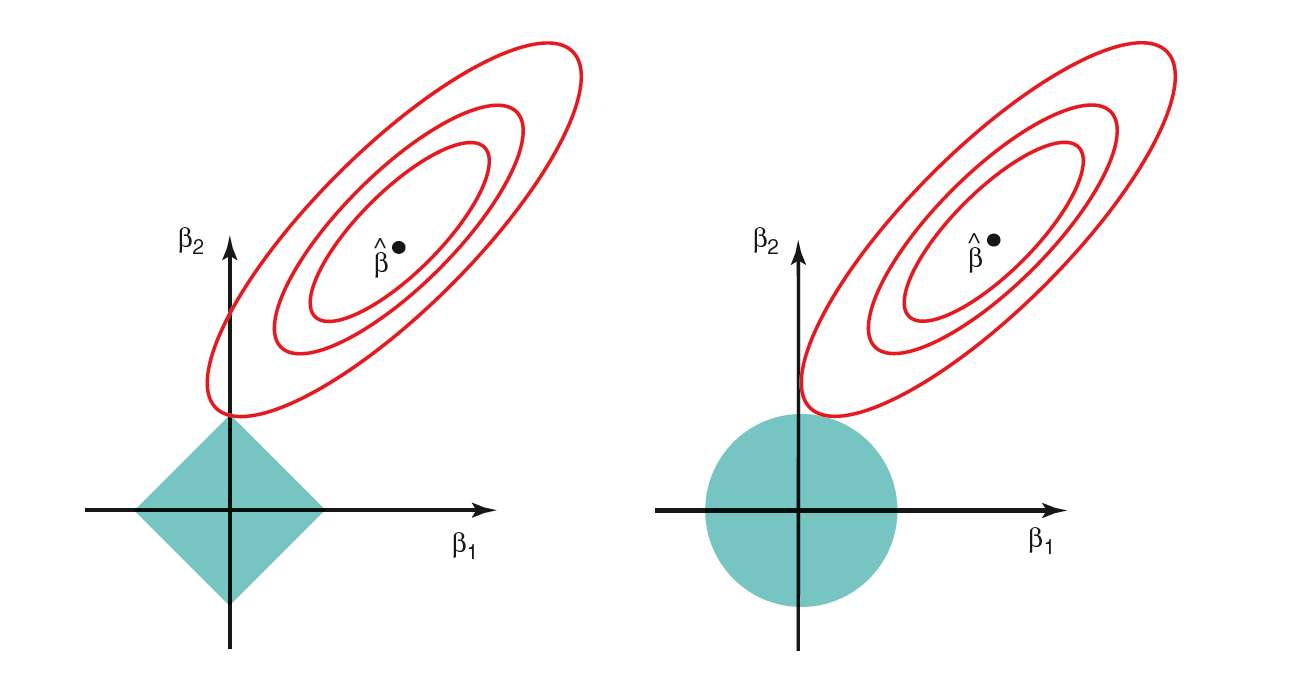
\includegraphics[width=.9\textwidth]{lasso.png}
\caption{Two types of regression regularization. On the left shows is LASSO regression, on the right is Ridge regression.  Figure from \citet{james2013}.}
\label{lasso}
\end{figure}

 
   \citet{casella08} suggested the Lasso estimates are comparable to the mode of the posterior distributions for the regression parameters when using identical Laplace priors. The prior on $\vec{\beta}$ is (setting the location parameter $\mu$ to zero):
  \begin{align}
p(\vec{\beta}| s) = \bigg(\frac{1}{2s}\bigg)^p \exp\left\{ -\frac{\sum\limits_{i=1}^p|\beta_i|}{s} \right\}
\label{laplace}
\end{align}
 
 \noindent When we combine the prior on $\vec{\beta}$ with a normal likelihood it becomes proportional to $\exp\bigg\{ (\vec{y}-\vec{X\beta})'(\vec{y}-\vec{X\beta}) -  \frac{1}{s}\sum \limits_{i=1}^p |\beta_i| \bigg\}$. Now $s$ is similar to the $\lambda$ penalty of the traditional LASSO approach.
 





\section{Markov chain Monte Carlo}

Bayesian inference is a method of statistical inference which uses Bayes' theorem to update probabilities of a hypothesis using data. Bayes' theorem is given as:
\begin{align}
\label{bayes}
P(A|B) =  \frac{ P(B |A) P(A) }{P(B)}.
\end{align}
 While Equation \ref{bayes} refers to simple, discrete events, it can be used to determine conditional densities as well. The conditional densities of interest are known as posterior densities which are of the following form:
\begin{equation}
\label{posterior}
\pi(\theta|x) = \frac{f(x|\theta) f(\theta)}{f(x)}
\end{equation}
where $f(x|\theta)$ is often referred to as the likelihood, $f(\theta)$ is known as the prior, and \newline $f(x)=\int_{\theta}f(x|\theta)f(\theta)d\theta$.

In the majority of statistical models, the posterior distribution in Equation \eqref{posterior} is only known up to the proportionality constant. This unknown proportionality prohibits calculation of posterior summaries such as the expectation, variance, and quantiles of interest. To overcome this obstacle, posterior summary statistics are calculated via Monte Carlo integration using a large sample from the posterior distribution. However, because the posterior distribution is often of unknown form, Markov chain Monte Carlo (MCMC) are a class of algorithms that can be used to sample from the posterior distribution \citep[see][]{robert04,gamerman06}.  While there are many MCMC algorithms, this section will focus on only one such algorithm: the Metropolis-Hastings algorithm \citep{metropolis53,hastings70,greenburg95}.

Let $\pi(\vec{\theta}\mid \vec{y})$ represent the posterior distribution of interest that can be evaluated for any value $\vec{\theta} \in \vec{\Theta}$ up to a proportionality constant. The Metropolis-Hastings algorithm is as follows: 
\begin{enumerate}
\item Choose a starting value: $\vec{\theta}_0$
\item For iteration $t=1,\dots,T$
\begin{enumerate}
\item Propose a new value by drawing $\vec{\theta}^\star \sim q_\sigma(\cdot\mid\vec{\theta}_{t-1})$ where $q_\sigma(\cdot\mid \vec{\theta}_{t-1})$ is a common density function (e.g.\ the normal) with scale parameter $\sigma$.  Note that the proposal distribution $q$ can depend on $\vec{\theta}_{t-1}$ but this does not necessarily have to be so.
\item Calculate the following ratio: 
\begin{align}
R = \frac{q_\sigma(\vec{\theta}_{t-1}\mid \vec{\theta}^\star)\pi(\vec{\theta}^\star\mid \vec{y})}{q_\sigma(\vec{\theta}^\star\mid \vec{\theta}_{t-1})\pi(\vec{\theta}_{t-1}\mid \vec{y})} 
\label{MH}
\end{align}
\item Set $\vec{\theta}_{t} = \vec{\theta}^\star$ with probability $\min(1,R)$.
\end{enumerate}
\end{enumerate}
Using properties of Markov chains, \citet{metropolis53} show that as $T\rightarrow \infty$ then draws $\vec{\theta}_{t}$ will resemble random vectors drawn from $\pi(\vec{\theta}\mid\vec{y})$.

In practice, having a proper proposal distribution $q_\sigma$ is key to obtaining draws from $\pi(\vec{\theta}\mid\vec{y})$ in a finite amount of time. Typically, a symmetric proposal density is used because  $R$ in \eqref{MH} reduces $ R = \pi(\vec{\theta}^\star)/\pi(\vec{\theta}_{t-1})$ since  $q_\sigma(\vec{\theta}_{t-1}\mid \vec{\theta}^\star) = q_\sigma(\vec{\theta}^\star\mid \vec{\theta}_{t-1})$  Even when $q_\sigma$ is symmetric, the choice of the scale parameter $\sigma$ is important: if $\sigma$ is too large then the Markov chain will rarely accept proposed values but a $\sigma$ too small will produce a chain that does not efficiently explore the space of the posterior distribution. For this reason, \citet{haario01} proposed using an adaptive metropolis algorithm.

Suppose at iteration $t$,  the chain has sampled points $\vec{\theta}_1,...,\vec{\theta}_{t-1}$. The adaptive algorithm of \citet{haario01} lets  $q_\sigma$ be a Gaussian distribution centered at the current point, with covariance matrix equal to $\vec{C}_t= (2.4^2/P)\times \text{Cov}(\vec{\theta}_1,...,\vec{\theta}_{t-1}) + (2.4^2/P) \epsilon I_P$ where $P$ is the dimension of $\vec{\theta}$.  The $\epsilon > 0$ is a chosen small constant and $I_P$ is a $P$-dimensional identity matrix. In practice, a starting covariance matrix $C_0$ is chosen and then choose an index $t_0 \in \{1,\dots,T\}$ such that: 
\begin{align*}
    C_t = 
\begin{cases}
    C_0 ,& \text{if } t\leq t_0\\
    \frac{2.4^2}{P}\times\text{Cov}(\vec{\theta}_1,...,\vec{\theta}_{t-1}) + \frac{2.4^2}{P} \epsilon I_P,              & t > t_0
\end{cases}
\end{align*}
The parameter $\epsilon$ must be greater than zero to ensure that the covariance matrix remains positive definite but $\epsilon$ is preferrably very small.




